Since there is no restriction on how the Kripke structure should look, we use
the one shown in Figure~\ref{figure:Figures_Kripke_Structure_Exercise_10}.

\begin{minipage}[t]{0.45\textwidth}
    \centering
    \captionof{figure}{A small Kripke structure}
    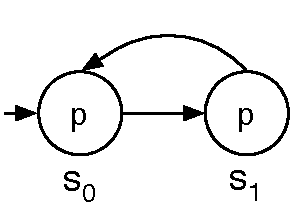
\includegraphics[width=.6\textwidth]
        {Figures/Kripke Structure Exercise 10.pdf}
    \label{figure:Figures_Kripke_Structure_Exercise_10}
\end{minipage}
\begin{minipage}[t]{0.45\textwidth}
    \vskip 1cm
    We use the LTL specification $s₀⊧X(X¬p)$. The smallest counterexample for
    this formula is $s₀, s₁, s₀$.
\end{minipage}
